\documentclass[tikz,border=15pt]{standalone}
\usepackage{amsmath}
\usetikzlibrary{arrows.meta,calc,angles,quotes,positioning}

\begin{document}
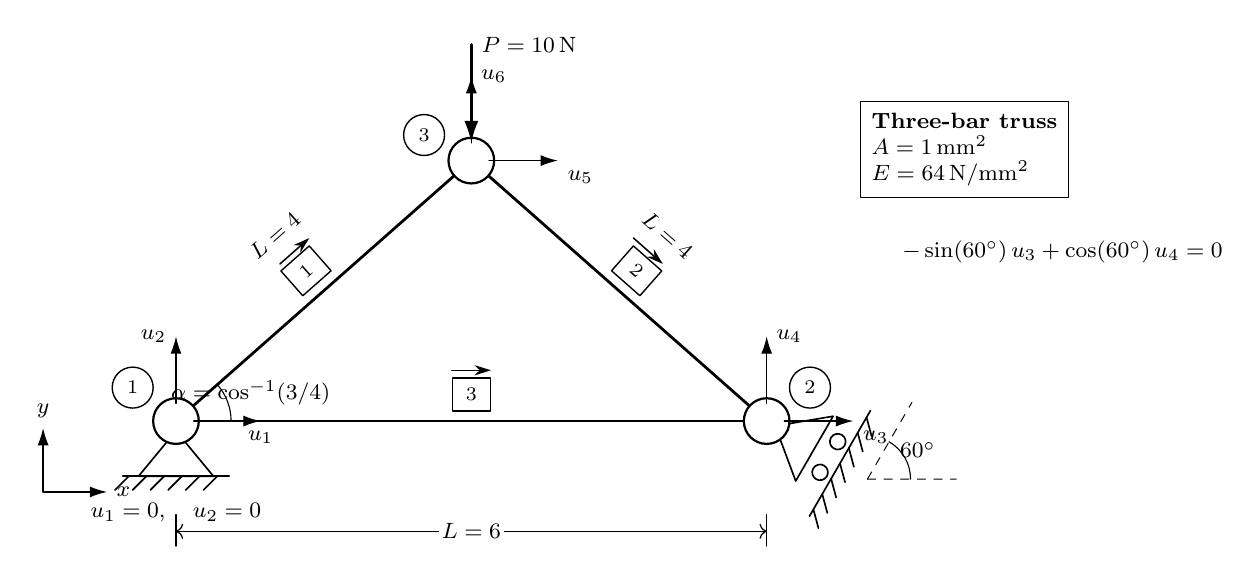
\begin{tikzpicture}[scale=1.25, font=\footnotesize, line cap=round, line join=round]
    \coordinate (N1) at (0,0);
    \coordinate (N2) at (6,0);
    \coordinate (N3) at (3,2.64575);

    \tikzset{
        truss/.style={draw=black, line width=1.0pt},
        joint/.style={circle, draw=black, fill=white, line width=0.8pt, minimum size=5.8mm, inner sep=0pt},
        elemLabel/.style={draw=black, fill=white, line width=0.5pt, minimum width=4.8mm, minimum height=4.2mm, inner sep=1pt, font=\scriptsize},
        nodeLabel/.style={circle, draw=black, fill=white, line width=0.5pt, minimum size=5.2mm, inner sep=0pt, font=\scriptsize},
        dof/.style={-{Latex[length=2.2mm,width=1.4mm]}, line width=0.5pt},
        load/.style={-{Latex[length=2.8mm,width=1.8mm]}, line width=0.9pt},
        guide/.style={draw=black, line width=0.6pt},
        dim/.style={draw=black, line width=0.45pt},
        note/.style={align=left}
    }

    \newcommand{\drawelement}[3]{%
        \draw[truss] (#1) -- (#2);
        \path (#1) -- (#2)
            node[midway, sloped, above=1.2mm, elemLabel] (E#3) {#3};
        \draw[-{Stealth[length=2.1mm,width=1.3mm]}, line width=0.55pt]
            ($(E#3.north west)+(0,0.7mm)$) -- ($(E#3.north east)+(0,0.7mm)$);
    }

    % Global axes
    \begin{scope}[shift={(-1.35,-0.72)}]
        \draw[dof] (0,0) -- (0.65,0) node[right] {$x$};
        \draw[dof] (0,0) -- (0,0.65) node[above] {$y$};
    \end{scope}

    % Node 1 pinned support
    \begin{scope}[shift={(N1)}]
        \draw[guide] (0,-0.10) -- (-0.38,-0.56) -- (0.38,-0.56) -- cycle;
        \draw[guide] (-0.54,-0.56) -- (0.54,-0.56);
        \foreach \x in {-0.48,-0.30,-0.12,0.06,0.24,0.42} {
            \draw[guide] (\x,-0.56) -- ++(-0.14,-0.14);
        }
    \end{scope}

    % Node 2 roller on a 60 degree incline
    \begin{scope}[shift={(N2)}, rotate=60]
        \draw[guide] (0,-0.10) -- (-0.38,-0.56) -- (0.38,-0.56) -- cycle;
        \draw[guide] (-0.18,-0.73) circle (0.08);
        \draw[guide] (0.18,-0.73) circle (0.08);
        \draw[guide] (-0.62,-0.86) -- (0.62,-0.86);
        \foreach \x in {-0.54,-0.36,-0.18,0,0.18,0.36,0.54} {
            \draw[guide] (\x,-0.86) -- ++(-0.14,-0.14);
        }
    \end{scope}

    % Angle of the inclined support
    \coordinate (G0) at ($(N2)+(-30:1.18)$);
    \coordinate (Gh) at ($(G0)+(0.9,0)$);
    \coordinate (Gp) at ($(G0)+(60:0.9)$);
    \draw[dashed, line width=0.35pt] (G0) -- (Gh);
    \draw[dashed, line width=0.35pt] (G0) -- (Gp);
    \pic [draw=black, angle radius=5.5mm, angle eccentricity=1.35, "$60^\circ$"] {angle = Gh--G0--Gp};

    % Truss members
    \drawelement{N1}{N3}{1}
    \drawelement{N3}{N2}{2}
    \drawelement{N1}{N2}{3}

    % Joints
    \node[joint] at (N1) {};
    \node[joint] at (N2) {};
    \node[joint] at (N3) {};

    % Node labels
    \node[nodeLabel] at ($(N1)+(-0.44,0.34)$) {1};
    \node[nodeLabel] at ($(N2)+(0.44,0.34)$) {2};
    \node[nodeLabel] at ($(N3)+(-0.48,0.26)$) {3};

    % Dimensions
    \draw[dim] ($(N1)+(0,-0.95)$) -- ++(0,-0.32);
    \draw[dim] ($(N2)+(0,-0.95)$) -- ++(0,-0.32);
    \draw[dim,<->] ($(N1)+(0,-1.12)$) -- ($(N2)+(0,-1.12)$)
        node[midway, fill=white, inner sep=1pt] {$L=6$};
    \path (N1) -- (N3) node[midway, sloped, above=8mm, fill=white, inner sep=1pt] {$L=4$};
    \path (N3) -- (N2) node[midway, sloped, above=8mm, fill=white, inner sep=1pt] {$L=4$};

    % Material box
    \node[draw=black, fill=white, inner sep=4pt, anchor=north west, note] at (6.95,3.25) {%
        \textbf{Three-bar truss}\\
        $A = 1\,\mathrm{mm}^2$\\
        $E = 64\,\mathrm{N/mm}^2$
    };

    % Constraints and load
    \node[note, anchor=north] at ($(N1)+(0.00,-0.74)$) {$u_1 = 0,\quad u_2 = 0$};
    \node[note, anchor=west] at ($(N2)+(1.28,1.72)$) {$-\sin(60^\circ)\,u_3 + \cos(60^\circ)\,u_4 = 0$};
    \draw[load] ($(N3)+(0,1.18)$) -- ($(N3)+(0,0.18)$)
        node[pos=0, right] {$P = 10\,\mathrm{N}$};

    % DOFs
    \draw[dof] ($(N1)+(0.18,0)$) -- ++(0.68,0) node[below] {$u_1$};
    \draw[dof] ($(N1)+(0,0.18)$) -- ++(0,0.68) node[left] {$u_2$};
    \draw[dof] ($(N2)+(0.18,0)$) -- ++(0.70,0) node[below right] {$u_3$};
    \draw[dof] ($(N2)+(0,0.18)$) -- ++(0,0.68) node[right] {$u_4$};
    \draw[dof] ($(N3)+(0.18,0)$) -- ++(0.70,0) node[below right] {$u_5$};
    \draw[dof] ($(N3)+(0,0.18)$) -- ++(0,0.68) node[right] {$u_6$};

    % Left angle annotation
    \pic [draw=black, angle radius=7mm, angle eccentricity=1.45, "$\alpha=\cos^{-1}(3/4)$"] {angle = N2--N1--N3};
\end{tikzpicture}
\end{document}
